\chapter{A Multi-Faceted NLP Analysis of Misinformation Spreaders in Twitter}
\label{ch:spreaders}
In the previous Chapter, \Autoref{ch:political}, we explored the role of negative sentiment in political dialogue on Twitter, focusing on how it influences user engagement and how negatively charged posts tend to have larger network penetration. In addition to the prevalence of negativity, a broader issue on social media concerns the spread of misinformation. This Chapter examines the characteristics of misinformation spreaders by comparing users who share content from trusted sources with those who amplify untrusted ones.

Social media has become deeply embedded in daily life worldwide, serving not only as a means of entertainment and communication but also as a primary channel for news consumption and information exchange. Its open and participatory nature, however, combined with the challenges of effective content moderation, has created fertile ground for the rapid dissemination of misinformation.

Our aim in this Chapter is to investigate the linguistic and behavioural patterns of users who share content from questionable sources, contrasting them with users who circulate information from reliable outlets. To this end, we analyse Twitter (X) accounts associated with potential misinformation spreaders and apply transformer-based models adapted for social media text. These include sentiment and emotion analysis, topic modelling using the model introduced in \Autoref{ch:tweet-topic}, and hate speech detection based on the model described in \Autoref{ch:hate-speech}.

The findings suggest that, although certain distinctions emerge between users who share misinformation and those who do not, the overall content they post does not exhibit substantial differences. This highlights the complexity of identifying misinformation spreaders based solely on textual features and underscores the importance of considering behavioural and contextual signals alongside linguistic ones.

This chapter reproduces verbatim our paper \textit{A Multi-Faceted NLP Analysis of Misinformation Spreaders in Twitter}, published at the 14th Workshop on Computational Approaches to Subjectivity, Sentiment, \& Social Media Analysis, 2024 (\Autoref{ch:intro:publications:parttwo}, \Autoref{publication:6}), with only minor modifications to presentation. It corresponds directly to the contributions outlined in \Autoref{ch:intro:contributions:part2}, specifically \Autoref{contribution:5}, \textit{Profiling Misinformation Spreaders}.

\section{Introduction}
The emerging popularity of social platforms such as Facebook, Twitter, and WhatsApp has revolutionised the way information is disseminated and consumed \cite{FacebookWorldwide, murthy2018twitter, deshmukh2015analysis}. People are able to express their sentiments, share their opinions on multiple topics, and to discuss and influence each other %\cite{barbieri2020tweeteval} 
with ease and at a speed that has transformed not only how we communicate but also how we perceive the world around us. Unfortunately, the capacity to reach a vast audience within seconds, along with the challenges that arise with verifying an ever-expanding volume of content, has created fertile ground within social media for malicious actors, or unaware users, to spread misinformation. The recent examples of fake news related to the COVID-19 pandemic \cite{evanega2020coronavirus}, and the ongoing war in Ukraine \cite{pierri2023propaganda} demonstrate that misinformation in social media is a complex problem with far-reaching implications for society, democracy, and information integrity.

Combating misinformation in social media is a topic that is studied extensively in academia \cite{vosoughi2018spread, pennycook2020implied} and in the natural language processing (NLP) community \cite{su2020motivations} specifically, among others. Common approaches of dealing with misinformation include defining the problem as a classification task \cite{serrano2020nlp, hamid2020fake} and classifying a post as fake or not; with fact-checking \cite{thorne2018automated} often defined as an information retrieval task \cite{lazarski2021using}. However, research regarding the agents that share misinformation is rather limited in comparison  \cite{shu2020fakenewsnet, rangel2020overview, dou2021user} particularly when it comes to analysing language-specific features.

In this Chapter, we focus on misinformation in Twitter and perform an analytical comparison between %trusted and unreliable 
different types of user based on their content shared online and the reliability of their sources.  %irrespective of its veracity.
To this end, we first compiled three diverse datasets in which spreaders of misinformation are categorised using different techniques. Then, we perform an exhaustive analysis of the content of these users by leveraging transformer-based language models specialised on social media tasks such as sentiment analysis, emotion recognition, topic categorisation and hate speech detection. The main contributions of this Chapter are the following: (1) we gather and consolidate existing and new Twitter datasets related to misinformation spreaders; and (2) we extract insights for the behaviour of such users in comparison with users sharing content from reliable sources.

\section{Related Work}

The study of identifying misinformation has been a prominent area of research in recent years. Initially, efforts focused on addressing the problem through classification, either in a binary or multiclass context. Some studies delved into examining the spread of true and false information online work on the topic of information dissemination \cite{vosoughi2018spread}. Meanwhile, others opted for a data mining approach in the realm of fake news detection on social media, utilising various features and machine learning algorithms to classify news articles as true or false \cite{shu2017fake}.

Moreover, beyond binary classification, researchers explored multiclass classification methods. For instance, \citet{castillo2011information} investigated the credibility of information on Twitter and proposed a framework categorizing tweets into four groups: true, false, unverified, and non-informative. \citet{zubiaga2016analysing} delved into the analysis of conversational threads on social media to gain insights into how rumors propagate and how individuals respond to them, shedding light on the dynamics of misinformation propagation.

These approaches evolved to better serve journalists and fact-checkers. The focus shifted from classification to fact-checking and information retrieval, aiming to assist journalists in source verification. This transition led to the development of tools to meet their specific needs \cite{schlichtkrull2023intended}. The availability of datasets like FEVER \cite{thorne2018fever}, MultiFC \cite{Augenstein2019multific}, and X-Fact \cite{gupta2021x} has been instrumental in enabling researchers to experiment with and develop novel methods for evidence retrieval and rumour verification \cite{nasir2021fake, lee2020language, lewis2020retrieval}.



While there have been notable studies in the broader field of misinformation and fact verification, there's a notable gap when it comes to a systematic analysis of the textual content of fake news spreaders. Much of the existing research has predominantly focused on the detection of misinformation sources, fact-checking, or the development of classification algorithms to distinguish true from false content. However, there is limited in-depth work that methodically dissects the text generated by those actively involved in spreading fake news that utilises state-of-the-art models \cite{ghanem2020factweet, rangel2020overview} and where the language analysis is not supplementary to the network and graph analysis \cite{aswani2019experience}. 

In this work we seek to methodically analyse the textual content generated by those responsible for spreading fake news. The primary objective is to gain a deeper understanding of the characteristics, strategies, and linguistic patterns employed by these actors in disseminating misleading or false information. Unlike traditional fact-checking, our work  does not intend to verify or debunk specific claims but rather aims at understanding the textual content shared by individuals or groups behind the spread of fake news, thereby providing further insights into their content dissemination strategies.


\section{Data}
\label{sec:data}
For our analysis, we exclusively focus on Twitter users, particularly tweets in the English language. Our goal was to extract a diverse tweet corpus for both users regularly spreading fake news or news from questionable sources, and users sharing content from verified sources. In the following we describe our data collection methodology stemming from various sources.


\subsection{Data Collection}
% \label{sec:data_collection}

In total, we draw upon three diverse data sources to extract relevant tweets from user account sharing trusted and untrusted sources. %(Section \ref{sec:mbfc} to \ref{sec:pan}). 
Moreover, we extract tweets from legacy-verified Twitter accounts as a control group. %(Section \ref{sec:control}).   %and (4) Twitter's API, which is utilized to extract verified users (\textit{Verified})\footnote{https://help.twitter.com/en/managing-your-account/about-twitter-verified-accounts}. 


\subsubsection{Media Bias Fact Check (MBFC)} 
\label{sec:mbfc}
Our first corpus is extracted from a list of known conspiracy sites provided by "Media Bias Fact Check" (\textit{MBFC}). This source is commonly used in the study of fake news \cite{nakov2020fact, cinelli2020covid}. For this dataset, we extracted tweets that share URLs from known untrusted sites\footnote{https://mediabiasfactcheck.com/conspiracy/} and then sample users based on the frequency of sharing these links. In particular, we considered only those users in the 75 percentile in terms of number of links shared. In order to gather enough information, all user accounts that were not older than 30 days were excluded from the analysis.  Subsequently, all posts made by the sampled users during September 2021 were collected, which aligns with the date when the \textit{MBFC} lists were last updated prior to conducting this experiment. User accounts were then further filtered based on their activity, only keeping those users posting more frequently than the median daily posts. %those posting less than the median daily posts being excluded. 
Finally, to ensure a diverse representation, users were sampled based on their number of followers by maintaining the original distribution and thus encompassing both popular and less popular accounts. This final sample represents the \textbf{\textit{MBFC-untrusted}} subset.

The above methodology is mirrored to collect users that share links form trusted news-sources according to MBFC\footnote{https://mediabiasfactcheck.com/pro-science/, https://mediabiasfactcheck.com/center/} resulting in the \textbf{\textit{MBFC-trusted}} subset.



\subsubsection{FakeNewsNet (FNN)} 
\label{sec:fnn}
The FakeNewsNet dataset, referred to as \textit{FNN} \cite{shu2020fakenewsnet}, contains two subsets: (1) tweets related to news content, e.g. tweets revolving around US politics and tweets; and (2) tweets related to social context, e.g. tweets talking about celebrities. Tweets in each groups are further classified as either untrusted  or trusted. For the purpose of this study, we concentrate solely on the politics-related subset, as it exhibits a closer alignment with the majority of the links found within the \textit{MBFC} lists. To extract relevant users, we initially scrape all tweets in the dataset and randomly sample users. Finally, all tweets posted by the selected users from September 2021 are retrieved. Only the accounts that have at least 100 posts were considered to create the \textbf{\textit{FNN-untrusted}} and \textbf{\textit{FNN-trusted}} subsets.


\subsubsection{Profiling Fake News Spreaders (PAN)}
\label{sec:pan}

The English subset of the \textit{PAN 2020: Profiling Fake News Spreaders} task (\textit{PAN}) \cite{rangel2020overview} is dataset that comprises a total of 50,000 English tweets obtained from 500 users, with each user contributing 100 tweets. These users are categorized as either trusted news spreaders (\textbf{\textit{PAN-trusted}}) or untrusted news spreaders (\textbf{\textit{PAN-untrusted}}). In the interest of privacy, no additional user-specific information, such as author descriptions or popularity metrics, is disclosed. Despite its relatively modest size and the limitation on the extraction of additional user details, the \textit{PAN} dataset is considered robust and reliable. Its construction involved manual checks, and it underwent thorough scrutiny by multiple individuals, primarily due to its relevance in a competitive context. This rigorous validation process enhances the dataset's trustworthiness and accuracy.


\subsubsection{Control (Verified users)}
\label{sec:Spreaders-control}

In order to have a control group to compare in our experiments, we sampled tweets from legacy-verified accounts for which the authenticity is known. This dataset was compiled by sampling verified users and collecting their tweets during the same time period as the previous datasets. Our aim was to select users whose characteristics align closely with the distribution patterns observed in the \textit{FNN} and \textit{MBFC} datasets.



\begin{table}[]
\centering
\scalebox{1}{
\begin{tabular}{llccccc}
\textbf{}                      &      & \textbf{Tweets} & \textbf{Users} & \textbf{Size} & \textbf{TTR}  & \textbf{\#emoji}  \\ \hline
\textbf{MBFC}                  & untrusted & 1,703,896       & 1,489          & 136             & 0.018     & 0.24      \\
\textbf{}                      & trusted & 1,676,615       & 1,535          & 132             & 0.021     & 0.26      \\ \hline
\multirow{2}{*}{\textbf{FNN}}  & untrusted & 246,107         & 430            & 122             &  0.036   & 0.19     \\
                               & trusted & 351,857         & 476            & 124             &  0.030    & 0.13       \\ \hline
\multirow{2}{*}{\textbf{PAN}}  & untrusted & 25,000          & 250            & 88              & 0.138     & 0.02      \\
                               & trusted & 25,000          & 250            & 88              & 0.149     & 0.13    \\ \hline
\multicolumn{2}{l}{\textbf{Verified users}} & 178,324         & 803            & 103             &  0.048    & 0.26      \\ \hline \hline
\multicolumn{2}{l}{\textbf{Total}}    & 4,206,799       & 5,233          &  123               &   0.014   & 0.24         
\end{tabular}
}
\caption{Number of tweets and users present in each dataset studied. The average size of the tweet (number of characters), along with the Type Token Ratio (TTR) and average emoji presence, are also reported.}
\label{tab:counts}
\end{table}



\begin{table*}[ht]
\begin{adjustbox}{width=\textwidth,center}
\begin{tabular}{cc|cc|cc|c}
\multicolumn{2}{c|}{MBFC}  & \multicolumn{2}{c|}{FNN}   & PAN             &          & \multirow{2}{*}{Verified} \\ \cline{1-6}
untrusted      & trusted           & untrusted        & trusted         & untrusted            & trusted     &                           \\ \hline
news      & tigray         & biden       & music        & trump           & film     & game                      \\
biden     & jisoo          & people      & hit          & realdonaldtrump & kobe     & thunderstorm              \\
vaccine   & ethiopia       & say         & play         & new             & season   & football                  \\
covid     & indiedev       & trump       & househunters & instyle         & styles   & season                    \\
border    & tigraygenocide & ebay        & dance        & webtalk         & spoilers & good                      \\
passport  & brexit         & marijuana   & trump        & post            & promo    & thank                     \\
australia & bts            & prohibition & biden        & impeachment     & date     & collision                 \\
mandate   & dior           & covid       & september    & publish         & trailer  & direction                 \\
                 
\end{tabular}
\end{adjustbox}
\caption{Top eight terms in each dataset according to lexical specificity.}
\label{tab:lexspec}
\end{table*}

\subsection{Statistics and Descriptive Analysis}

 By considering these diverse data sources, we aim to comprehensively examine and understand the dynamics of untrusted news spreaders on the Twitter platform. Our analysis encompasses a total of 4,206,799 tweets contributed by 5,233 users, as presented in Table \ref{tab:counts}. In addition to the number of tweets and users, we also investigate the average length of tweet and average emoji usage. We did not identify a clear pattern between the \textit{trusted} and \textit{untrusted} subsets as far as these metrics are concerned. 


Looking into the lexical characteristics of each dataset, distinctions between the \textit{untrusted} and \textit{trusted} subsets become more apparent. For instance, when assessing lexical diversity using the Type Token Ratio (TTR), we observe that \textit{untrusted} users, with the exception of the \textit{FNN} dataset, tend to employ a less diverse vocabulary which is consistent with previous research \cite{horne2017just}. %Additionally, 
Our analysis based on the average presence of emojis in each tweet reveals no consistent pattern, despite prior research suggesting higher emoji usage among untrusted news spreaders \cite{jarnas1087772}. For example, while the untrusted subset of the MBFC dataset exhibits higher emoji usage, the opposite holds true for the FNN dataset.



\paragraph{Lexical specificity.} To gain an overall understanding of the prevalent topics within our corpora, we employ lexical specificity \cite{lafon1980variabilite}. Lexical specificity is a word-level metric that indicates the importance of each word in a subcorpus. In particular, for this analysis we use the formulation outlined in \citeauthor{camacho2016nasari} (\citeyear{camacho2016nasari}), and extract the top terms in each dataset. Table \ref{tab:lexspec} displays the top ten lemmas\footnote{Lemmatization was done using \textit{spaCy} https://spacy.io/.} in each dataset based on their lexical specificity scores.
%\cite{githubGitHubExplosionspaCy} 


Notably, due to the same time period during data collection, a significant overlap exists between the \textit{MBFC} and \textit{FNN} datasets, particularly within their 'untrusted' subsets. Terms such as 'biden' and 'vaccine' are common across both. Additionally, a discernible trend emerges, indicating that 'untrusted' subsets across datasets often feature more controversial and divisive topics. This is evident in the presence of terms like 'covid,' 'prohibition,' and 'impeachment,' in contrast to the 'trusted' subsets, which exhibit more generic and neutral terms such as 'bts,' 'music,' and 'film.' This distinction becomes even more pronounced when examining the top terms in the \textit{Verified} dataset, which include terms like 'game,' 'football,' and 'love.'


\section{Methodology}
\label{sec:methodology}
Our goal is to analyse various content-related features from the extracted posts in Section \ref{sec:data}. To capture the nuanced language features present in the data, we employ a range of pre-trained language models designed for social media usage.  Our primary focus encompasses sentiment and affection analysis, topic classification, and the identification of hate speech in textual content, features are frequently employed in the study of misinformation propagation \cite{vicario2019polarization, verma2020understanding}, aiming to uncover emotionally charged language and controversial topics.

All the language models used are built upon the RoBERTa architecture \cite{ROBERTA} and trained on social media corpora, making them well-suited for analysing Twitter data. More specifically:
%\begin{itemize}
    \paragraph{Sentiment Analysis.} The model \textit{twitter-roberta-base-sentiment-latest} \cite{loureiro-etal-2022-timelms} is used to extract the sentiment polarity where each tweet is classified as \textit{negative, neutral, or positive}. This model has been fine-tuned for sentiment analysis using the dataset provided in the \textit{Sentiment Analysis in Twitter} task of Semeval 2017 \cite{rosenthal2017semeval}.  By analysing the sentiment expressed in social media content, we can gain insights into information being shared  \cite{101007s42979021009189}. Specifically, presence of exaggerated positive sentiment or negative sentiment in response to fake news can serve as indicators of misinformation  \cite{electronics10111348}. 
    
    \paragraph{Emotion Analysis.} We leverage \textit{twitter-roberta-base-emotion-multilabel-latest} \cite{camacho2022tweetnlp} to assign one or more emotions to each tweet. This model is trained using data from the 'Affect in Tweets' Semeval 2018 task \cite{mohammad2018semeval}, covering 11 different emotions. Similar to sentiment analysis, the presence of specific emotions has been used to analyse the spread of rumours and misinformation, with negative emotions potentially contributing to the spread of misinformation \cite{vosoughi2018spread, weeks2015emotions}.
    
    
    \paragraph{Hate Speech Detection.} We use the \textit{twitter-roberta-base-hate-multiclass} hate speech detection model \cite{antypas2023robust}, which is trained on a combination of 13 different hate speech Twitter datasets and is capable of identifying hate speech from seven target groups. The inclusion of hate speech detection as a feature is motivated by previous research indicating a positive correlation between the presence of hate speech and misinformation \cite{10117720563051221150410}. 


\begin{figure}[!ht]
\centering
\scalebox{0.9}{
  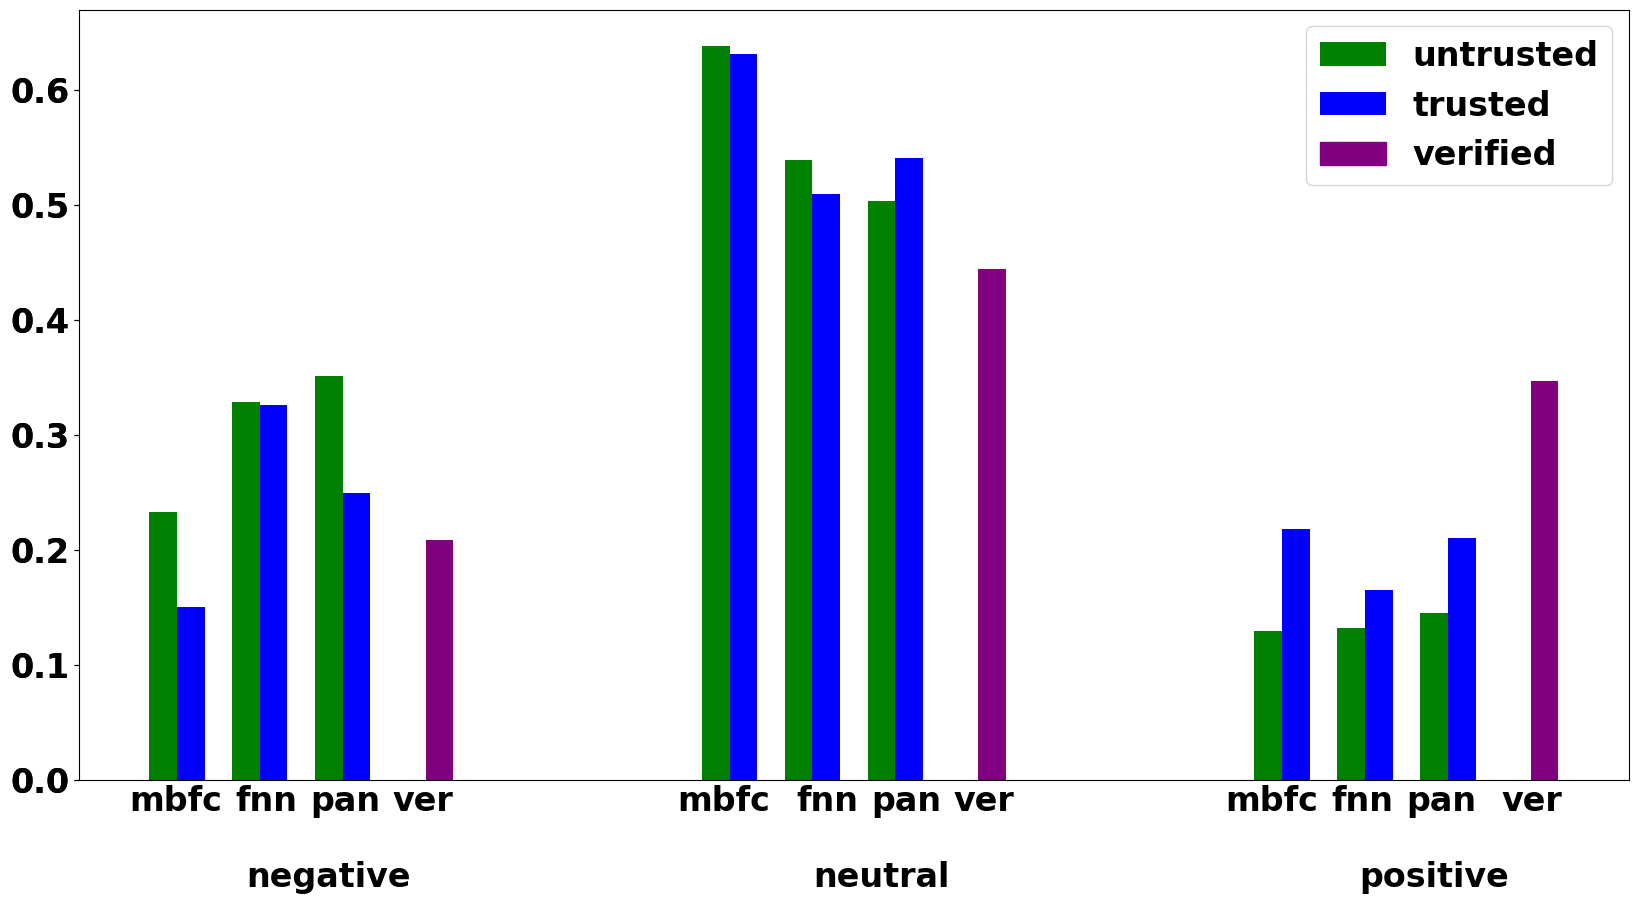
\includegraphics[width=\textwidth]{../figures/spreaders/sentiment.png}
}
\caption{Sentiment distribution in each dataset for \textit{trusted} and \textit{untrusted} users in Twitter.}
\label{fig:sentiment-distribution}
\end{figure}


    \paragraph{Topic Classification.} We use \textit{tweet-topic-21-multi} \cite{antypas2022twitter}, a multi-label classification model fine-tuned on a Twitter topic classification dataset. This model assigns one or more topics to each tweet from a list of 19 topics. Our hypothesis is that there may be a significant difference between the topics discussed by \textit{untrusted} news spreaders and regular users, e.g. untrusted news spreaders potentially engaging in discussions related to sensitive topics at a higher volume.
    
%\end{itemize}

All the specialised models described above are perform in line of the state of the art for each of the tasks in the social media context\footnote{Sentiment Analysis: 73.7\% Recall, Emotion Analysis: 80\% F1-macro, Hate Speech: 94\% Accuracy, Topic Classification: 59\% F1-macro -- please refer to the individual references for more details.} and they enable us to delve deeper into the complex linguistic nuances within the social media data. Nonetheless, as we describe in the Limitations section, they all have a degree of error that needs to be considered when making conclusions.




\begin{table*}
\centering
\begin{adjustbox}{width=\textwidth,center}
\begin{tabular}{llll|ll|ll|l}
 & \multirow{2}{*}{} & \multicolumn{2}{c|}{MBFC} & \multicolumn{2}{c|}{PAN} & \multicolumn{2}{c|}{FNN} & \multicolumn{1}{c}{\multirow{2}{*}{verified}} \\ \cline{3-8}
 &  & \multicolumn{1}{c}{untrusted} & \multicolumn{1}{c|}{trusted} & \multicolumn{1}{c}{untrusted} & \multicolumn{1}{c|}{trusted} & \multicolumn{1}{c}{untrusted} & \multicolumn{1}{c|}{trusted} & \multicolumn{1}{c}{} \\ \hline
\multirow{3}{*}{\begin{turn}{90}Senti.\end{turn}} & negative & 0.35 ± 0.12 & 0.32 ± 0.15 & 0.16 ± 0.14 & 0.24 ± 0.16 & 0.35 ± 0.19 & 0.37 ± 0.19 & 0.2 ± 0.11 \\
 & neutral & 0.52 ± 0.1 & 0.5 ± 0.11 & 0.63 ± 0.18 & 0.64 ± 0.15 & 0.48 ± 0.18 & 0.47 ± 0.17 & 0.44 ± 0.15 \\
 & positive & \multicolumn{1}{c}{0.13 ± 0.09} & \multicolumn{1}{c|}{0.17 ± 0.12} & \multicolumn{1}{c}{0.22 ± 0.17} & \multicolumn{1}{c|}{0.13 ± 0.09} & \multicolumn{1}{c}{0.17 ± 0.15} & \multicolumn{1}{c|}{0.16 ± 0.14} & \multicolumn{1}{c}{0.37 ± 0.16} \\ \hline
\multirow{11}{*}{\begin{turn}{90}Emotion\end{turn}} & anger & 0.39 ± 0.14 & 0.34 ± 0.17 & 0.1 ± 0.11 & 0.21 ± 0.17 & 0.33 ± 0.24 & 0.37 ± 0.23 & 0.17 ± 0.11 \\
 & anticipation & 0.25 ± 0.1 & 0.26 ± 0.12 & 0.48 ± 0.2 & 0.38 ± 0.18 & 0.28 ± 0.19 & 0.26 ± 0.19 & 0.28 ± 0.12 \\
 & disgust & 0.42 ± 0.15 & 0.37 ± 0.17 & 0.12 ± 0.12 & 0.23 ± 0.18 & 0.35 ± 0.23 & 0.39 ± 0.23 & 0.18 ± 0.11 \\
 & fear & 0.1 ± 0.05 & 0.09 ± 0.08 & 0.06 ± 0.08 & 0.08 ± 0.07 & 0.09 ± 0.09 & 0.1 ± 0.12 & 0.04 ± 0.05 \\
 & joy & 0.2 ± 0.12 & 0.26 ± 0.17 & 0.46 ± 0.22 & 0.34 ± 0.22 & 0.26 ± 0.2 & 0.24 ± 0.19 & 0.46 ± 0.16 \\
 & love & 0.02 ± 0.03 & 0.03 ± 0.05 & 0.04 ± 0.06 & 0.02 ± 0.03 & 0.03 ± 0.05 & 0.03 ± 0.05 & 0.07 ± 0.07 \\
 & optimism & 0.16 ± 0.1 & 0.19 ± 0.11 & 0.19 ± 0.14 & 0.12 ± 0.1 & 0.18 ± 0.14 & 0.18 ± 0.14 & 0.31 ± 0.14 \\
 & pessimism & 0.01 ± 0.01 & 0.01 ± 0.01 & 0.01 ± 0.02 & 0.01 ± 0.01 & 0.01 ± 0.01 & 0.01 ± 0.01 & 0.01 ± 0.01 \\
 & sadness & 0.09 ± 0.04 & 0.1 ± 0.05 & 0.07 ± 0.06 & 0.08 ± 0.05 & 0.1 ± 0.07 & 0.1 ± 0.09 & 0.09 ± 0.05 \\
 & surprise & 0.01 ± 0.01 & 0.01 ± 0.01 & 0.01 ± 0.01 & 0.01 ± 0.01 & 0.01 ± 0.01 & 0.01 ± 0.01 & 0.02 ± 0.01 \\
 & trust & 0.0 ± 0.0 & 0.0 ± 0.0 & 0.0 ± 0.0 & 0.0 ± 0.0 & 0.0 ± 0.0 & 0.0 ± 0.0 & 0.0 ± 0.0 \\ \hline
\multirow{6}{*}{\begin{turn}{90}Hate\end{turn}} & disability & 0.0 ± 0.0 & 0.0 ± 0.0 & 0.0 ± 0.0 & 0.0 ± 0.0 & 0.0 ± 0.0 & 0.0 ± 0.0 & 0.0 ± 0.0 \\
 & not\_hate & 0.99 ± 0.01 & 0.99 ± 0.01 & 1.0 ± 0.01 & 1.0 ± 0.01 & 0.99 ± 0.01 & 0.99 ± 0.02 & 1.0 ± 0.0 \\
 & other & 0.0 ± 0.0 & 0.0 ± 0.0 & 0.0 ± 0.0 & 0.0 ± 0.0 & 0.0 ± 0.0 & 0.0 ± 0.0 & 0.01 ± 0.0 \\
 & racism & 0.01 ± 0.01 & 0.01 ± 0.01 & 0.02 ± 0.01 & 0.02 ± 0.02 & 0.01 ± 0.01 & 0.01 ± 0.02 & 0.01 ± 0.01 \\
 & sexism & 0.01 ± 0.01 & 0.01 ± 0.01 & 0.02 ± 0.01 & 0.02 ± 0.01 & 0.01 ± 0.01 & 0.01 ± 0.01 & 0.01 ± 0.0 \\
 & religion & 0.0 ± 0.0 & 0.0 ± 0.0 & 0.03 ± 0.0 & 0.01 ± 0.0 & 0.0 ± 0.0 & 0.0 ± 0.0 & 0.01 ± 0.0 \\
 & sex\_orient & 0.0 ± 0.0 & 0.0 ± 0.0 & 0.0 ± 0.0 & 0.01 ± 0.0 & 0.0 ± 0.0 & 0.0 ± 0.0 & 0.0 ± 0.0 \\ \hline
\multirow{19}{*}{\begin{turn}{90}Topic\end{turn}} & arts & 0.01 ± 0.03 & 0.02 ± 0.03 & 0.04 ± 0.1 & 0.02 ± 0.02 & 0.02 ± 0.05 & 0.02 ± 0.08 & 0.01 ± 0.03 \\
 & business & 0.06 ± 0.11 & 0.05 ± 0.1 & 0.07 ± 0.11 & 0.06 ± 0.1 & 0.05 ± 0.11 & 0.04 ± 0.1 & 0.02 ± 0.05 \\
 & celebrity & 0.05 ± 0.04 & 0.07 ± 0.08 & 0.24 ± 0.21 & 0.28 ± 0.28 & 0.05 ± 0.05 & 0.05 ± 0.08 & 0.07 ± 0.07 \\
 & diaries & 0.07 ± 0.07 & 0.09 ± 0.09 & 0.08 ± 0.1 & 0.04 ± 0.07 & 0.08 ± 0.1 & 0.08 ± 0.11 & 0.15 ± 0.1 \\
 & family & 0.01 ± 0.01 & 0.01 ± 0.01 & 0.01 ± 0.02 & 0.01 ± 0.01 & 0.01 ± 0.01 & 0.01 ± 0.01 & 0.01 ± 0.01 \\
 & fashion & 0.0 ± 0.01 & 0.01 ± 0.02 & 0.06 ± 0.13 & 0.05 ± 0.1 & 0.01 ± 0.01 & 0.01 ± 0.02 & 0.01 ± 0.01 \\
 & film & 0.03 ± 0.03 & 0.04 ± 0.05 & 0.23 ± 0.26 & 0.16 ± 0.18 & 0.04 ± 0.06 & 0.05 ± 0.09 & 0.06 ± 0.07 \\
 & fitness & 0.11 ± 0.11 & 0.06 ± 0.07 & 0.02 ± 0.04 & 0.02 ± 0.03 & 0.05 ± 0.07 & 0.06 ± 0.07 & 0.02 ± 0.04 \\
 & food & 0.01 ± 0.02 & 0.02 ± 0.03 & 0.02 ± 0.05 & 0.01 ± 0.02 & 0.02 ± 0.04 & 0.02 ± 0.03 & 0.03 ± 0.03 \\
 & gaming & 0.0 ± 0.02 & 0.0 ± 0.02 & 0.01 ± 0.02 & 0.01 ± 0.03 & 0.0 ± 0.02 & 0.0 ± 0.02 & 0.01 ± 0.04 \\
 & learning & 0.02 ± 0.03 & 0.03 ± 0.04 & 0.01 ± 0.02 & 0.02 ± 0.02 & 0.03 ± 0.06 & 0.03 ± 0.07 & 0.02 ± 0.04 \\
 & music & 0.02 ± 0.03 & 0.03 ± 0.07 & 0.09 ± 0.14 & 0.08 ± 0.13 & 0.04 ± 0.13 & 0.04 ± 0.11 & 0.04 ± 0.06 \\
 & news & 0.76 ± 0.2 & 0.67 ± 0.27 & 0.31 ± 0.27 & 0.51 ± 0.29 & 0.65 ± 0.3 & 0.68 ± 0.27 & 0.24 ± 0.22 \\
 & hobbies & 0.01 ± 0.03 & 0.01 ± 0.02 & 0.01 ± 0.02 & 0.0 ± 0.01 & 0.01 ± 0.04 & 0.01 ± 0.03 & 0.01 ± 0.01 \\
 & relations & 0.01 ± 0.01 & 0.01 ± 0.02 & 0.02 ± 0.03 & 0.02 ± 0.03 & 0.01 ± 0.01 & 0.01 ± 0.02 & 0.01 ± 0.02 \\
 & science & 0.05 ± 0.07 & 0.04 ± 0.08 & 0.04 ± 0.11 & 0.05 ± 0.09 & 0.04 ± 0.06 & 0.04 ± 0.08 & 0.02 ± 0.04 \\
 & sports & 0.03 ± 0.05 & 0.06 ± 0.13 & 0.08 ± 0.15 & 0.08 ± 0.11 & 0.08 ± 0.15 & 0.05 ± 0.1 & 0.35 ± 0.31 \\
 & travel & 0.01 ± 0.01 & 0.01 ± 0.02 & 0.02 ± 0.07 & 0.01 ± 0.01 & 0.02 ± 0.04 & 0.01 ± 0.02 & 0.02 ± 0.05 \\
 & youth & 0.02 ± 0.02 & 0.02 ± 0.03 & 0.01 ± 0.01 & 0.01 ± 0.02 & 0.02 ± 0.06 & 0.01 ± 0.02 & 0.01 ± 0.02
\end{tabular}
\end{adjustbox}
\caption{Average presence of each feature (i.e., sentiment analysis, emotion analysis, hate speech, and topic classification) per user along with standard deviations.}
\label{tab:results}
\end{table*}

\section{Analysis}
We consider each pair of collected datasets (\textit{untrusted} and \textit{trusted}), along with the \textit{Verified} control dataset. Our examination involves a comparison of the tweets within each dataset individually, as well as their aggregation for each user. This holistic approach enables us to explore a variety of perspectives and insights across the datasets and their combined impact.

\subsection{Textual Analysis}
Table \ref{tab:results} displays the aggregated results for the sentiment, emotion, hate speech and topic analysis. For each feature we consider each user independently by taking their mean value and then aggregate the results of users belonging in the same subset. Even though differences between \textit{untrusted} and \textit{trusted} subsets exist, it is challenging to identify trends that are consistent across the datasets. In the following sections we investigate each  characteristic individually. 


% \begin{figure*}
%   \begin{subfigure}{0.5\textwidth}
%     \centering
%     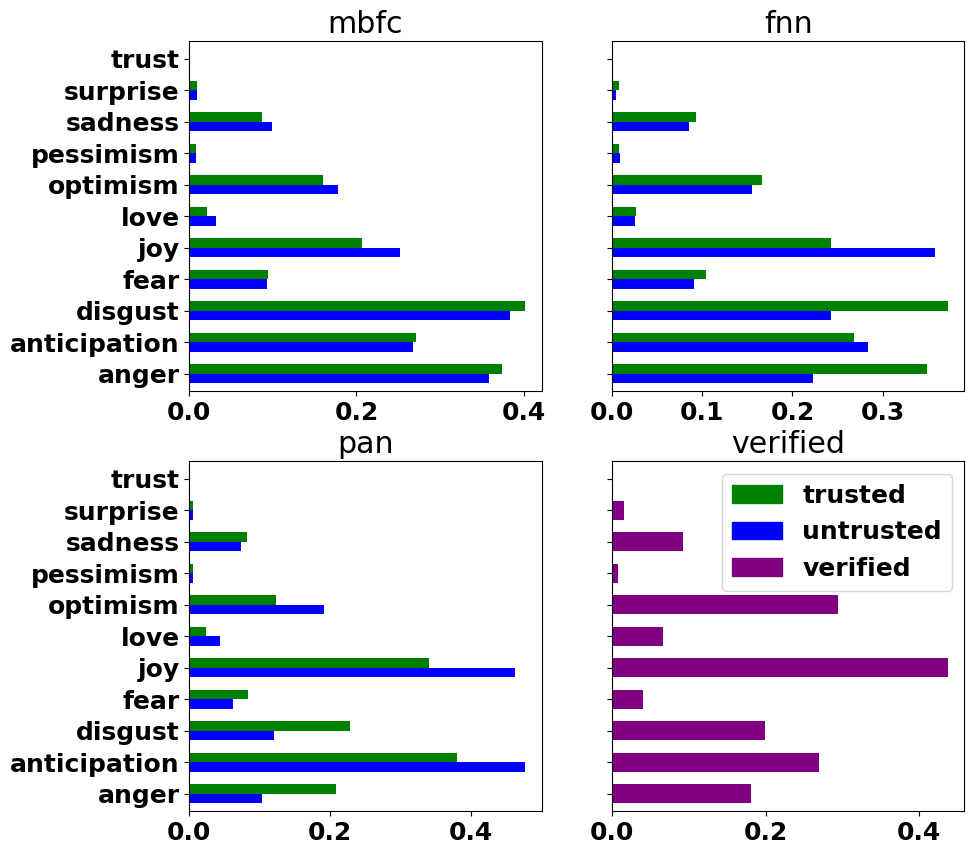
\includegraphics[width=\linewidth]{../figures/spreaders/emotions.png}
%     \caption{Emotion distribution in each dataset.}
%     \label{fig:emotion-distribution}
%   \end{subfigure}%
%   \begin{subfigure}{0.5\textwidth}
%     \centering
%     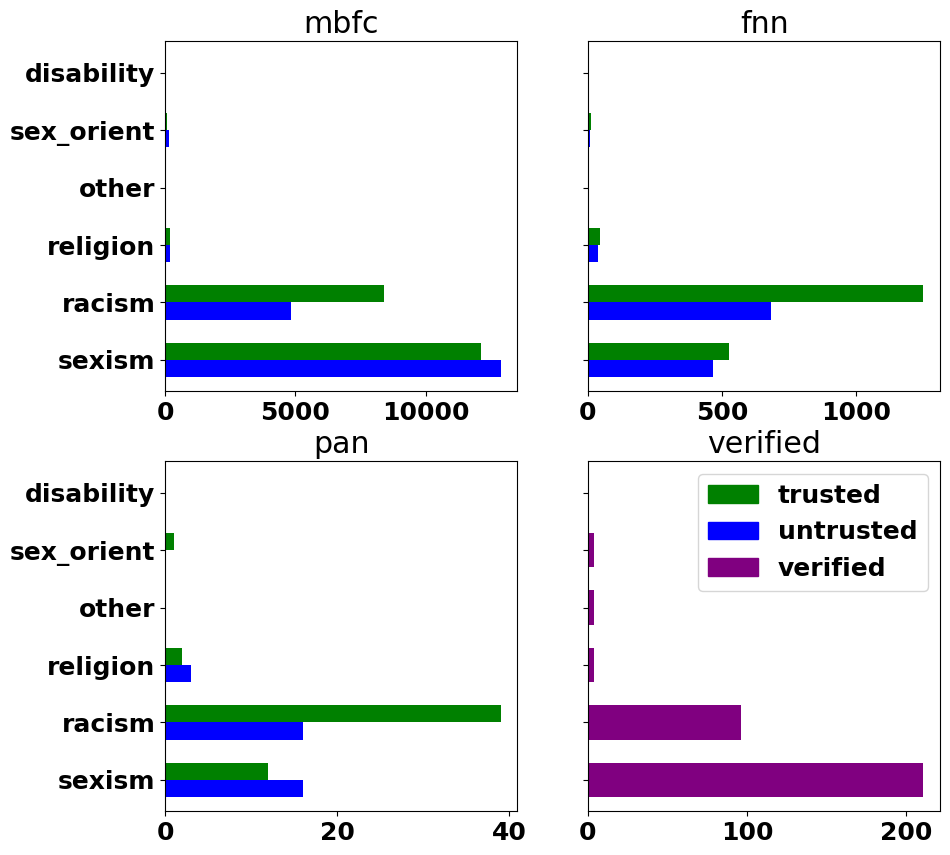
\includegraphics[width=\linewidth]{../figures/spreaders/hate.png}
%     \caption{Hateful entries in each dataset.}
%     \label{fig:hate-distribution}
%   \end{subfigure}
%   \caption{Emotion \& Hate speech results of \textit{trusted} and \textit{untrusted} users in Twitter.}
% \end{figure*}
  
\subsubsection{Sentiment}
When evaluating the presence of sentiment in tweets, a noticeable trend emerges: tweets associated with \textit{untrusted} news spreaders tend to exhibit a higher degree of negativity compared to those posted by other users. The distribution of sentiment across the datasets is displayed in Figure \ref{fig:sentiment-distribution}. In the case of the \textit{FNN} dataset, however, this difference is almost not negligible. Finally, even though there is more negativity in \textit{untrusted} users, the distributions among negative, neutral and positive tweets are very similar in all cases except for the verified users that tend to be more positive overall.

\begin{figure*}[!t]
  \centering
  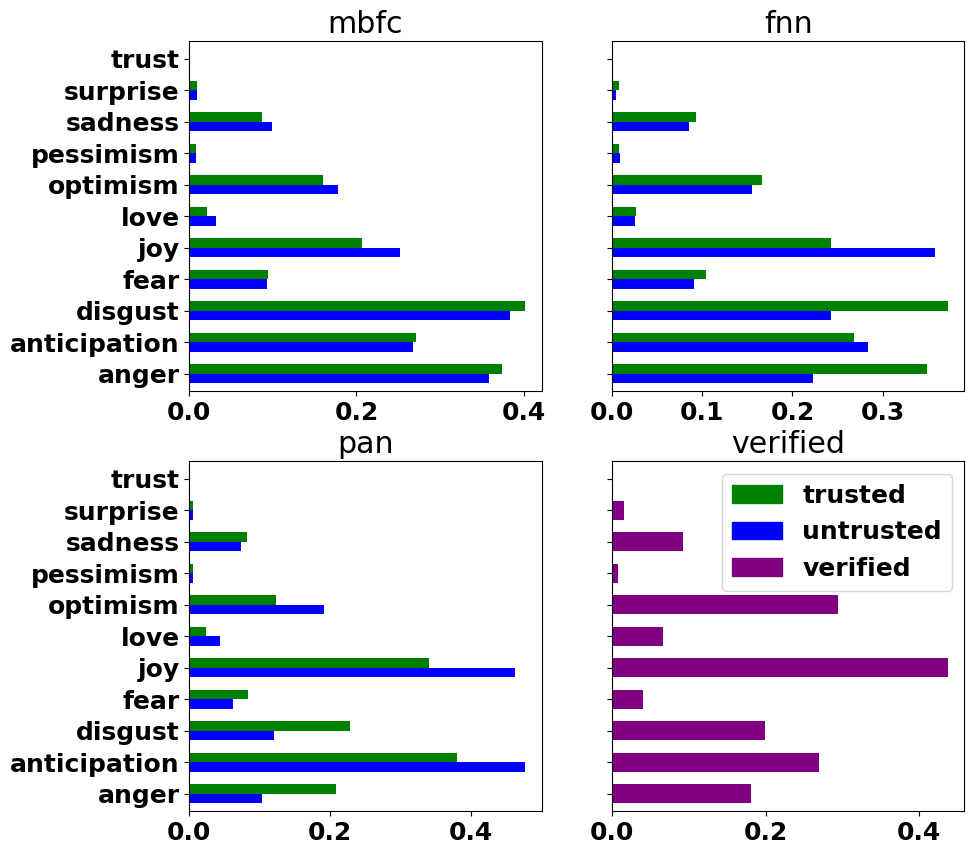
\includegraphics[width=1\linewidth]{../figures/spreaders/emotions.png}
  \caption{Emotion distribution in each dataset.}
  \label{fig:emotion-distribution}
\end{figure*}

\begin{figure*}[!t]
  \centering
  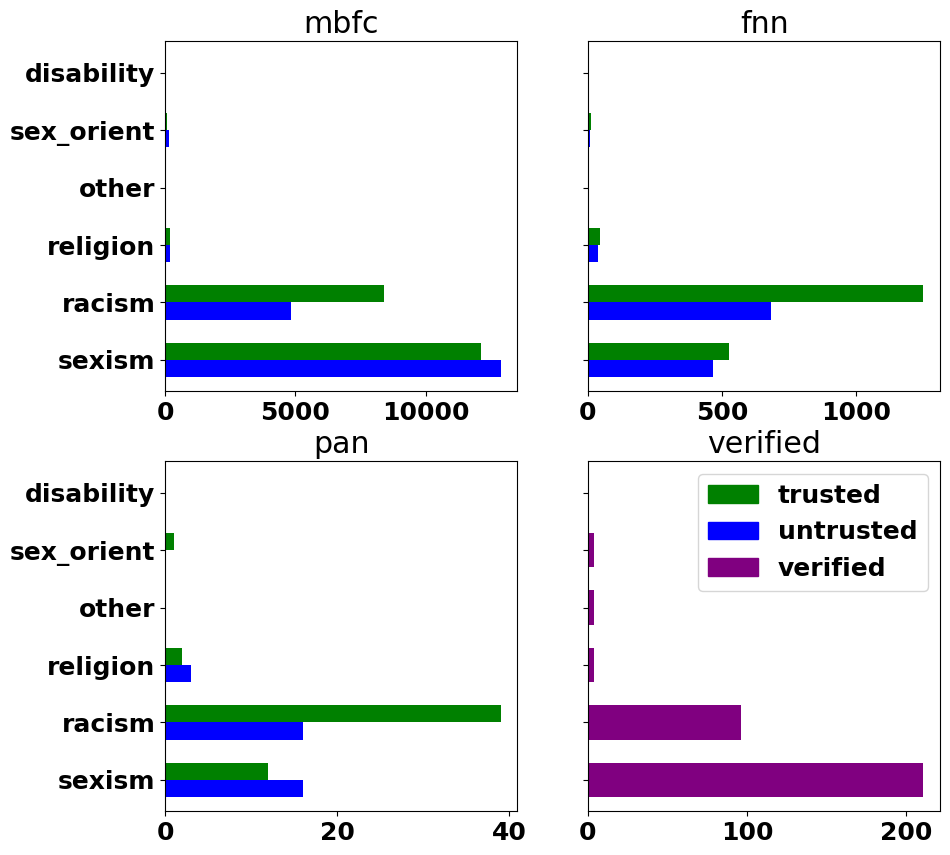
\includegraphics[width=1\linewidth]{../figures/spreaders/hate.png}
  \caption{Hateful entries in each dataset.}
  \label{fig:hate-distribution}
\end{figure*}


\subsubsection{Emotion}
Similarly to the findings in sentiment analysis, the analysis of affect reveals a consistent pattern where untrusted news spreaders tend to gravitate toward more negative emotions. Figure \ref{fig:emotion-distribution} provides insight into the distribution of the 11 emotions present across across all subsets.

A clear contrast emerges, with tweets attributed to \textit{trusted} users generally displaying greater joy and featuring a lesser presence of anger and disgust, in stark contrast to the tweets originating from \textit{untrusted} users. This trend remains consistent even when evaluating the per-user aggregation. Finally, similarly to the sentiment distribution patterns, there are no noticeable differences when analysing the overall emotion distribution and, in this case, it also related to that of verified users. %The results consistently underscore the distinct emotional tendencies of untrusted news spreaders in comparison to genuine users.

\subsubsection{Hate Speech}
When examining hate speech, a feature that often coexists with misinformation  \cite{10117720563051221150410}, such as Holocaust denial and the Great Replacement theory, it does not appear to be a prominent feature in the collected datasets. Our analysis indicates an absence of hate speech, with 99\% of all tweets being devoid of it.

There does appear to be a variance in the types of hate speech across the subsets (as displayed in Figure \ref{fig:hate-distribution}). \textit{Untrusted} subsets exhibit a higher inclination towards racism, while in the trusted subset, sexism appears to be more prevalent. However, given the limited number of instances, it is prudent to exercise caution when drawing extensive conclusions based on this data.


\subsubsection{Topics}


\begin{figure}[!ht]
\centering
\scalebox{1}{
  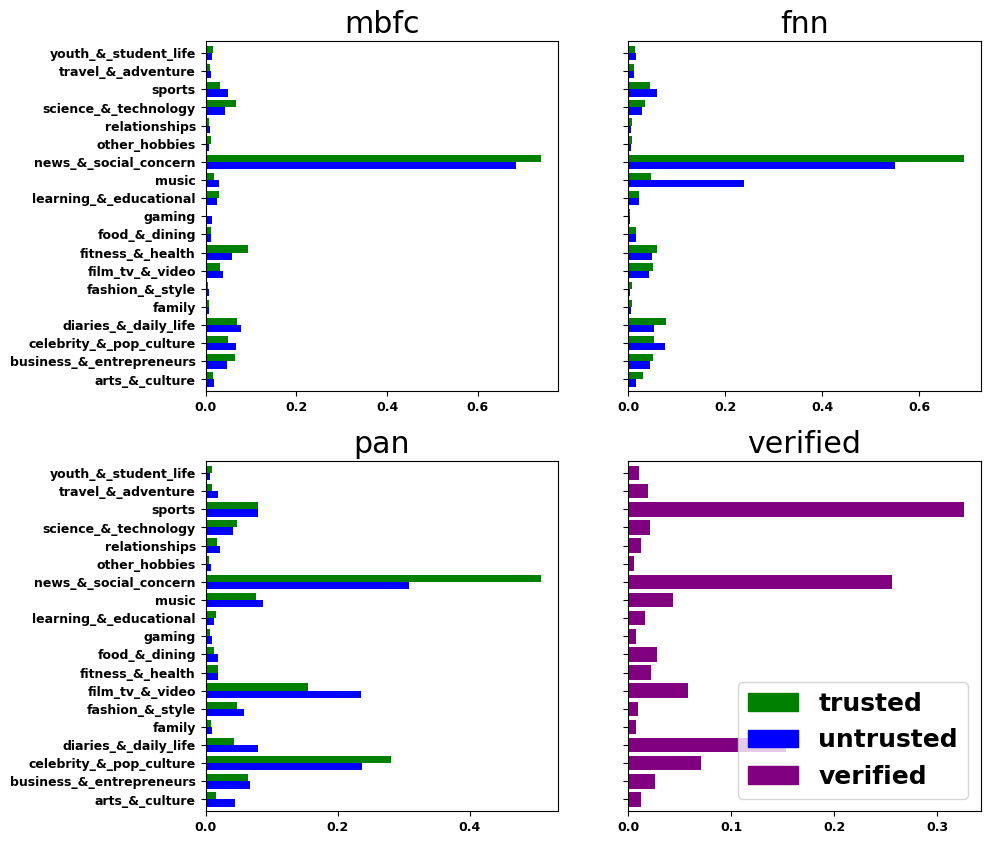
\includegraphics[width=\textwidth]{../figures/spreaders/topics.png}
}
\caption{Topic distribution in each dataset for \textit{trusted} and \textit{untrusted} users in Twitter.}
\label{fig:topics-distribution}
\end{figure}


% \begin{figure}[!ht]
% \centering
% \scalebox{0.7}{
%  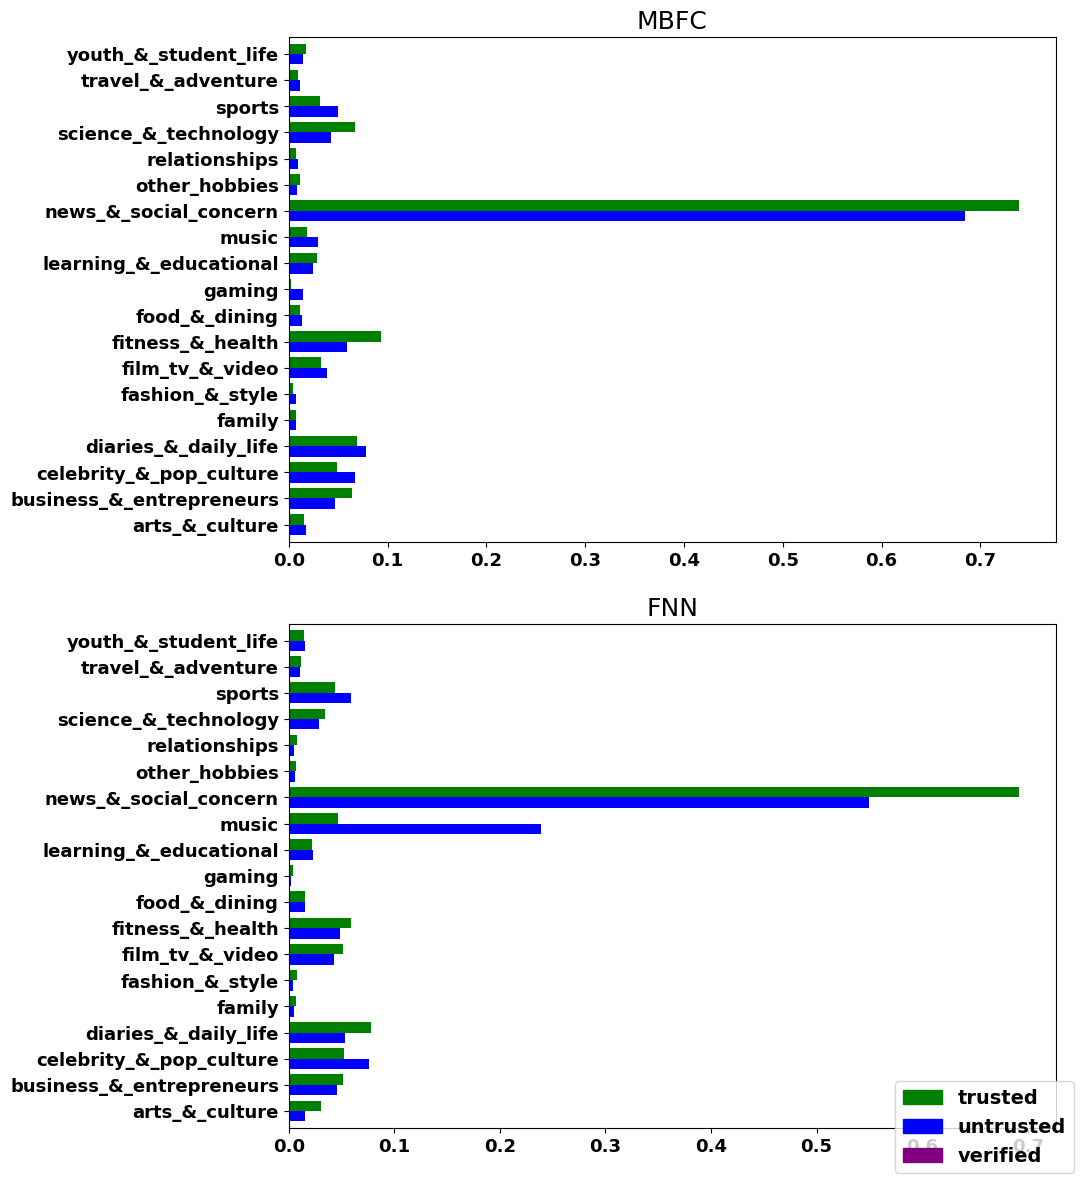
\includegraphics[width=\textwidth]{../figures/spreaders/topics_1.png}
% }
% \caption{Topic distribution for \textit{mbfc} and \textit{pan} users in Twitter.}
% \label{fig:topics-distribution1}
% \end{figure}

% \begin{figure}[!ht]
% \centering
% \scalebox{0.5}{
%   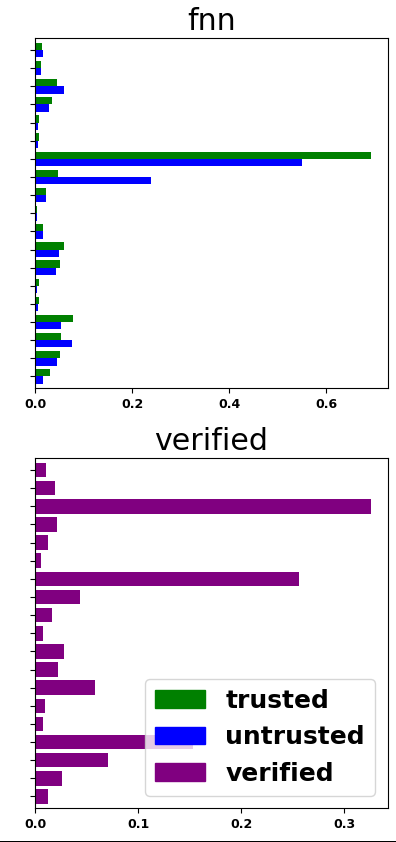
\includegraphics[width=\textwidth]{../figures/spreaders/topics_2.png}
% }
% \caption{Topic distribution for \textit{fnn} and \textit{verified} users in Twitter.}
% \label{fig:topics-distribution2}
% \end{figure}


Regarding the topics that \textit{untrusted} news spreaders and regular users typically discuss, the results appear to suggest a similar distribution of topics (Figures \ref{fig:topics-distribution1} \& \ref{fig:topics-distribution2}). \textit{Untrusted} news spreaders appear to engage more extensively in posting tweets related to news and social issues,  which are those related to politics, among others. This suggests that these accounts may be more socially active, and can create the illusion of a larger representation than that of the general population.

Conversely, there is no discernible distinction in the case of the remaining popular topics, with variations existing among the datasets. For instance, the topic "celebrity\_\&\_pop\_culture" is more prevalent in the \textit{Pan\-untrusted} dataset but less common in the other untrusted subsets. Again here we can observe more differences with respect to verified users, where \textit{sports} and \textit{diaries\_\&\_daily\_life} topics are much more prominent.

\subsection{Spreader Detection Analysis} \label{sec:detection-analysis}

Recognising that a significant portion of our datasets relies on weak labels, with the distinction between users propagating untrusted news and those who do not being based on heuristics based on the number of posts shared from untrusted sources, we perform a robustness analysis on the \textit{Pan20} dataset which includes train and test splits. To this end, we train a classifier capable of discerning between the \textit{trusted} and \textit{untrusted} classes and compare the results with our approach.

The train/test split originally utilised in the competition is retained, consisting of 300 users for training and 200 users for testing. We assess the performance of two classifiers: (1) A classifier based on the best-performing models as presented in the competition \cite{buda2020ensemble, pizarro2020}, utilising an XGBoost classifier \cite{chen2016xgboost}. This model is trained using TFIDF features and a combination of word and character n-grams; and (2) A pre-trained Longformer \cite{beltagy2020longformer}, which is further fine-tuned using the \textit{PAN} dataset. We leverage the implementation provided by Hugging Face \cite{wolf-etal-2020-transformers} for the fine-tuning of the Longformer\footnote{https://huggingface.co/allenai/longformer-base-4096}. Hyper-parameter tuning, including batch size, epochs number, and learning rate, is conducted using Ray Tune \cite{liaw2018tune}.

The results reveal that the XGBoost model (\textit{XGB}) surpasses the Longformer classifier, achieving a 74\% macro F1 score compared to the Longformer's 70\%. One possible explanation for this outcome lies in the unstructured nature of Twitter text, which presents an added challenge to the language model. The Longformer, not explicitly trained on social media corpus data, may face limitations in handling this specific type of text.


When examining the results of the XGB classifier  in the \textit{PAN} dataset, we observe an almost identical trend when compared with our initial results. For example, when looking the sentiment distribution of user accounts using the XGB classifier and our initial distinction of \textit{trusted} and \textit{untrusted} users, only minimal differences can be observed (\textit{Pan-untrusted}: 23\% Negative and 13\% Positive; \textit{XGB-untrusted}: 24\% and 13\%).

Our experiment indicates that even though developing a classifier to identify \textit{untrusted} users may not be the optimal approach, it can still be used as a proxy to derive useful information and identify patterns that can be used to reveal malicious actors. 
Additional results for all tasks regarding the performance of the \textit{XGB} model and the differences with our approach follow a similar trend and can be found in Appendix \ref{appendix:xgb}.

As a final experiment, we attempt to enhance our XGB classifier by integrating the features already extracted. Our results %(Appendix \ref{appendix:xgb})
reveal that while the incorporation of new features generally results in only marginal variations in the model's performance, the addition of certain features, especially sentiment, holds the potential to notably improve its effectiveness. This suggests that careful selection and integration of specific features can yield incremental but meaningful gains in the classifier's performance, an exploration that we leave for future work as it falls out of the scope of this work.


\section{Conclusion}
This Chapter's comparative analysis aims to delve into the dynamics of misinformation dissemination in the digital age by examining the distinctions between untrusted news spreaders and other users. To this end, we have compiled a substantial sample of untrusted news spreaders and the general content shared of these users in Twitter. Using this large corpus stemming from three diverse datasets (MBFC, FNN and PAN), we have analysed the disparities in their language usage.

The initial exploration of traits associated with untrusted news spreaders, including the presence of hate speech, did not necessarily reveal the distinctions we anticipated. Other language features such as sentiment and emotional content indicate the existence of relatively small language differences between the two groups of users. These differences provide valuable insights that can inform the development of systems designed to identify and counteract malicious accounts. In particular, our results suggest that misinformation mitigation efforts should be focused on the specific content shared, rather than in profiling individual accounts.

\section{Limitations}
\label{sec:limitations}
While we strived to derive insights from a large dataset using state-of-the-art classifiers and a robust analytical setup, we acknowledge the presence of factors that constrain the depth of our findings. For example, the focus on English-language content, potentially limiting the scope of global social media interactions and perspectives. Additionally, the exclusive use of Twitter data might not fully represent the dynamics on other social media platforms. While verified accounts are employed as a control group, it should be noted that they may not serve as a perfect control due to factors like their popularity, potential biases, or unique behaviours. Furthermore, the extraction of users relies on heuristics, introducing some degree of noise and potential inaccuracies in the data. Finally, we made use of automatic models based on transformers. While these have been tested extensively in prior work, there are inherent limitations in these models, as well as possible unwanted biases. All these limitations should be considered when interpreting our results and conclusions.


\section{Ethical Statement}
\label{sec:ethics}
In our study involving user-generated content from social media, we ensured user privacy in several ways. First, we replaced all user mentions in the texts with placeholders and removing user IDs. Moreover, all the data utilised in our research is sourced from publicly available information or collected using the official Twitter API. Finally, all the information is provided in an aggregated fashion, without reporting sensitive information from individual users.

While our dataset and methodology have the potential for analysing individual behaviours, our primary objective is to offer researchers a valuable tool for the analysis and aggregation of social media content.



